\documentclass[11pt,a4paper,oneside]{article}


\usepackage[utf8]{inputenc}
\usepackage{amsmath}
\usepackage{amsfonts}
\usepackage{amssymb}
\usepackage{graphicx}
\author{Igo Ramalho Brilhante \and Tales Parente}

\newcommand{\HRule}{\rule{\linewidth}{0.5mm}}

% BEFORE SUBMITTING FOR REVIEW, PLEASE:
% 1. Run a spell-checker:
% 2. Check anonymity constraints, if needed:
% 3. Change chato-notes to hide:
%\usepackage[showx]{style/chato-notes}
\usepackage[show]{../extras/chato-notes}



\newcounter{uc-counter} \setcounter{uc-counter}{1}
\newenvironment{uc}[1][]{\medskip\noindent \textbf{Caso de Uso \arabic{uc-counter}} -- \textbf{#1}}{\medskip \stepcounter{uc-counter}}

\begin{document}

\newcommand{\ucform}[9][]{
\begin{itemize}
	\item Identificador: #2
	\item Nome: #3
	\item Descrição: #4
	\item Prioridade: #5
	\item Fluxo de eventos:
						\begin{itemize}
							\item Fluxo principal: #6
							\item Fluxo de exceção: #7
						\end{itemize}
	\item Pré-condições e restrições: #8
	\item Pós-condições: #9
\end{itemize}
}

\begin{titlepage}
\begin{center}

% Upper part of the page. The '~' is needed because \\
% only works if a paragraph has started.

\includegraphics[scale=0.3]{figuras/brasao_ufc.jpg}~\\[1cm]

\textsc{\LARGE Universidade Federal do Ceará}\\[1.5cm]

\textsc{\Large Recomenda AI - \textsc{RAI}}\\[0.5cm]

% Title
\HRule \\[0.4cm]
{ \huge \bfseries Documento de Requisitos}\\[0.4cm]

\HRule \\[1.5cm]

% Author and supervisor
\begin{minipage}{0.4\textwidth}
\begin{flushleft} \large
\emph{Equipe:}\\
Igo \textsc{Brilhante}\\
Tales \textsc{Parent}
\end{flushleft}
\end{minipage}
%\begin{minipage}{0.4\textwidth}
%\begin{flushright} \large
%\emph{Professores:} \\
%Dr.~Mark \textsc{Brown}
%\end{flushright}
%\end{minipage}

\vfill

% Bottom of the page
{\large Junho 2013}

\end{center}
\end{titlepage}

\section{Introdução}
\note{Introduzir o sistema, aplicação móvel e servidor}

\section{Definição de Requisitos do Usuário}
\note{O que o usuário pode fazer com o sistema proposto}

\section{Arquitetura de Sistemas}
\note{Descrever a arquitetura}

\section{Especificação de Requisitos do Sistema}

\subsection{Requisitos Funcionais}
Os requisitos funcionais são:
\begin{itemize}
\item Cadastrar usuário;
\item Buscar locais mais próximos;
\item Ver condições climáticas;
\item Buscar recomendação;
\item Avaliar item da recomendação.
\end{itemize}

\subsection{Requisitos Não-Funcionais}
Os requisitos não funcionais são:
\begin{itemize}
\item Dispositivo móvel equipado com sistema opercional \emph{Android} versão mínima $2.3.3$. Além disso o celular deve ser equipado com sensor de GPS e conectividade wireless (WiFi, GSM, 3G, 3G+ ou 4G);
\item O sistema deve ter uma interface intuitiva com o usuário, apresentando menus simples e diretos para facilitar a utilização da aplicação;
\item O sistema deve gerenciar da melhor forma possível o uso da bateria do dispositivo.
\end{itemize}

\section{Casos de Uso}
\subsection{Visão Geral}

\begin{figure}
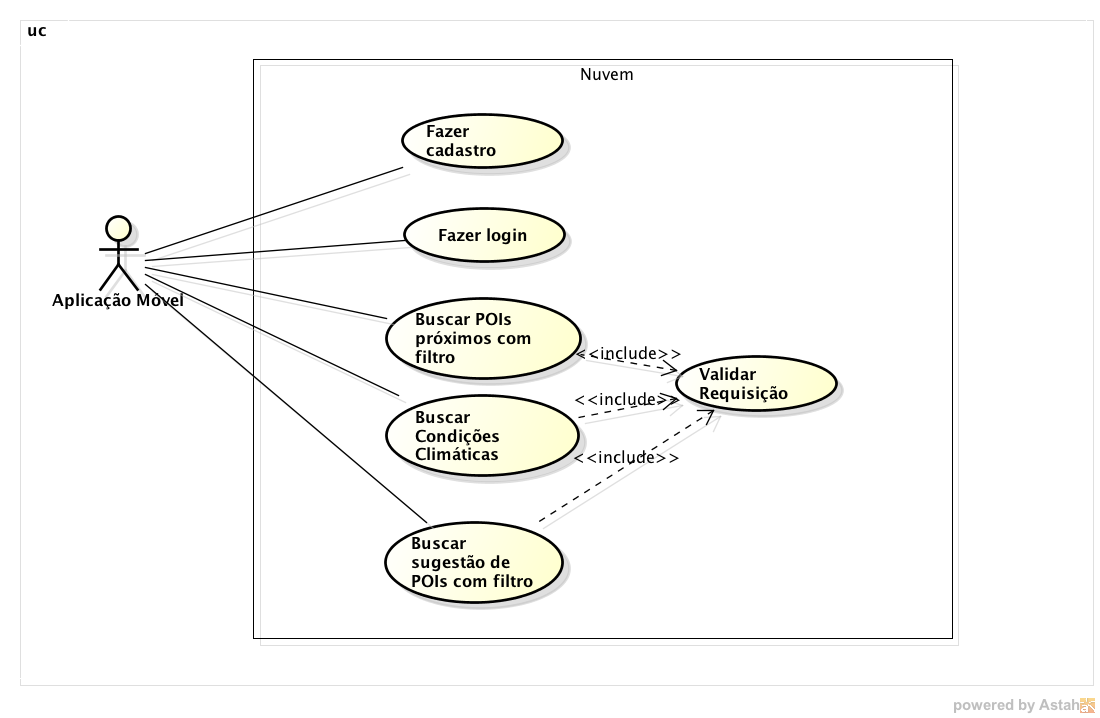
\includegraphics[scale=0.5]{../casos-de-usos/casos-de-usos-app-servidor.png}

\caption{Casos de usos para o ator \emph{aplicação móvel}.}
\label{fig:casos-de-usos-app-servidor}
\end{figure}

\subsection{Atores}
Os atores envolvidos no sistema são:
\begin{description}
\item \textbf{Usuário}. Usuário da aplicação móvel que busca informações ao seu redor bem como recomendações de pontos de interesses na cidade de Fortaleza;
\item \textbf{Aplicação Móvel}. A aplicação móvel é um ator para o consumo de serviços oferecidos pela nuvem.
\end{description}

\subsection{Casos de Usos}
\begin{uc}[Cadastrar usuário]
\ucform
{Cadastrar usuário}
{Cadastra usuário no sistema}
{Aplicação envia um \emph{username} e uma \emph{senha} para cadastrar um usuário}
{Essencial}
{Aplicação envia os dados para a nuvem}
{Aplicação não se comunidade com a nuvem}
{Aplicação deve está com acesso à Internet}
{Aplicação recebe confirmação de cadastro realizado com sucesso}
\end{uc}

\begin{uc}[Buscar locais mais próximos]
\ucform
{Buscar locais mais próximos}
{Buscar os locais mais próximos a uma da posição espacial}
{Buscar os locais que estão mais próximos a uma dada posição espacial}
{Essencial}
{Aplicação envia requisição de um usuáro com informação de contexto (posição espacial, tempo)}
{Aplicação não se comunidade com a nuvem}
{Aplicação deve está com acesso à Internet e está com sensor de posicionamento habilitado}
{Aplicação recebe uma lista de locais}
\end{uc}
%

\begin{uc}[Recomendar locais]
\ucform
{Recomendar locais}
{Recomendar locais relevantes para o usuário}
{Recomendar uma lista de locais para o usuário considerando o contexto}
{Essencial}
{Aplicação envia requisição de um usuáro com informações de contexto}
{Aplicação não se comunidade com a nuvem}
{Aplicação deve está com acesso à Internet e está com sensor de posicionamento habilitado}
{Aplicação recebe uma lista de locais recomendados a serem visitados}
\end{uc}

%
\begin{uc}[Buscar condições climáticas]
\ucform
{Buscar condições climáticas}
{Buscar condições climáticas de um local}
{Buscar condições climáticas de um dado local referente a um local na cidade}
{Essencial}
{Aplicação envia requisição de um usuáro com informações de contexto (posição espacial, tempo)}
{Aplicação não se comunidade com a nuvem}
{Aplicação deve está com acesso à Internet e está com sensor de posicionamento habilitado}
{Aplicação recebe informações sobre as condições climáticas}
\end{uc}

\section{Modelos de Sistemas}

\section{Evolução de Sistema}

\end{document}